\chapter{Contexto}
\label{chap:contexto}

\lettrine{E}{n} este apartado se introduce el contexto relevante a este trabajo que provee los conceptos básicos necesarios para su comprensión.
Para ello se describe el campo de la oftalmología y la imagen médica, así como el estado del arte en alineamiento de imágenes.

\section{Oftalmología}
\label{sec:Oftalmoloxía}
La oftalmología es la especialidad médica encargada del estudio y tratamiento de las enfermedades de los ojos, incluyendo el globo ocular, su musculatura, el sistema lagrimal y los párpados.
El ojo humano es uno de los órganos de los que más dependemos y mayor cantidad de información sensorial aporta, así como uno de los más complejos de nuestro cuerpo \cite{kanski2011clinical}.

La importancia de la oftalmología radica no solo en el tratamiento de las enfermedades oculares, sino también en su capacidad para proporcionar información valiosa sobre el estado de salud general del paciente.
La observación directa de los vasos sanguíneos y del tejido neuronal 'in vivo' permite a los oftalmólogos detectar signos precoces de diversas enfermedades sistémicas.
Por ejemplo, el glaucoma, que no presenta síntomas en sus etapas iniciales, puede ser diagnosticado mediante exámenes regulares de la presión ocular y del nervio óptico \cite{importglaucoma}.
Esta capacidad de diagnóstico precoz hace de la oftalmología una especialidad fundamental en la prevención y en el mantenimiento de la salud visual y general del paciente.

\subsection{Anatomía del ojo humano}
\label{subsec:Anatomía do ollo humano}
El ojo se encarga de captar la luz y transformarla en impulsos eléctricos que se envían al cerebro.
Esta información es interpretada por el cerebro, que mediante mecanismos como la atención y la memoria, permite la percepción visual. \cite{eyefunct}
El ojo humano está compuesto por varias estructuras, cada una con una función específica que permite la percepción visual \cite{eyeanat}. Entre ellas destacan:

\begin{itemize}
\item Córnea y Cristalino: actúan juntas para enfocar la luz en la retina. La córnea, situada en la parte exterior del ojo, proporciona mayor parte de la capacidad refractiva, mientras que el cristalino, una lente flexible, ajusta el enfoque para objetos a diferentes distancias.
\item Pupila e Iris: regulan la cantidad de luz que entra en el ojo. El iris, la parte coloreada del ojo, se expande o contrae para controlar el tamaño de la pupila, el orificio central.
\item Retina: una capa de células sensibles a la luz (fotorreceptores) que convierten los estímulos luminosos en señales eléctricas, procesados inicialmente en la retina misma.
\item Nervio óptico: transporta las señales eléctricas generadas en la retina hasta el cerebro, donde se interpretan como imágenes.
\item Disco óptico: también conocido como "punto ciego", es el área donde el nervio óptico sale del ojo; carece de fotorreceptores.
\item Vasos sanguíneos: distribuyen los nutrientes y el oxígeno necesarios a la retina y eliminan sus residuos metabólicos.
\end{itemize}

La figura \ref{fig:imaxes_ojo} muestra estas estructuras localizadas en imágenes.

\begin{figure}[tbp]
    \centering
    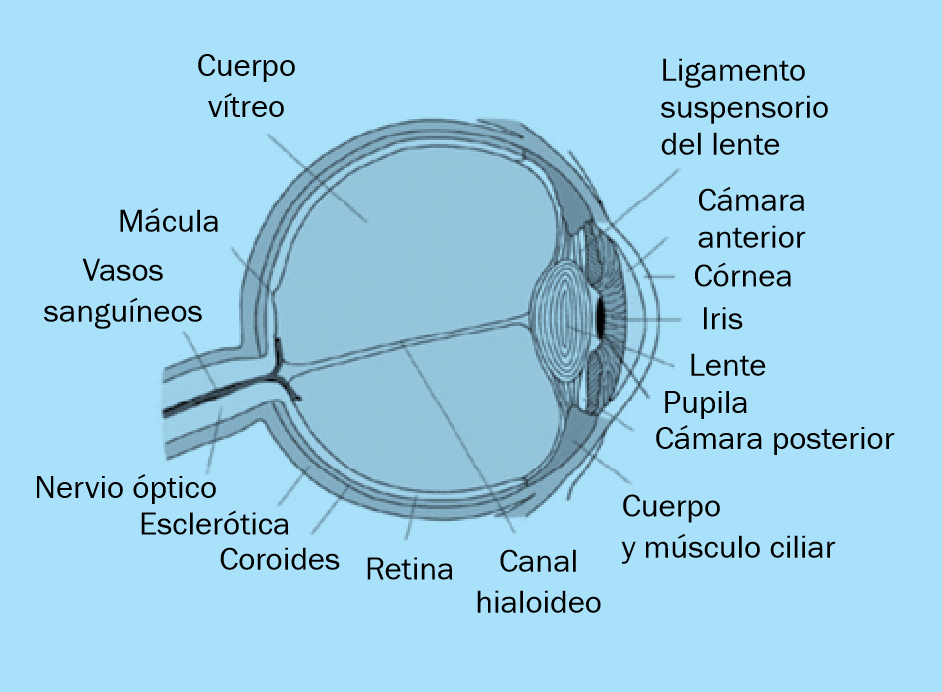
\includegraphics[width=0.45\textwidth]{imaxes/ojo1.png}
    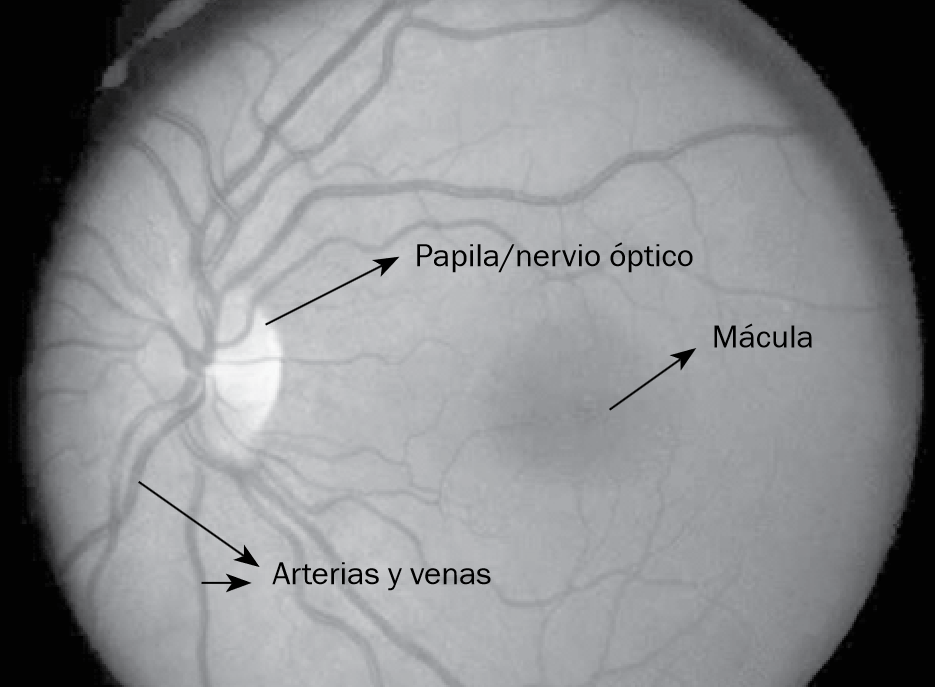
\includegraphics[width=0.45\textwidth]{imaxes/ojo2.png}
    \caption{Imágenes del ojo humano, extraídas de \cite{visionyojo}. A la izquierda, vista lateral del ojo anotada. A la derecha, retinografía del ojo anotada.}
    \label{fig:imaxes_ojo}
\end{figure}

\subsection{Imagen oftalmológica}
\label{subsec:Imaxe oftalmolóxica}
Existen diversas modalidades de imagen médica que permiten observar el ojo, cada una con diferentes propiedades y aplicaciones.
Entre ellas se incluyen la fotografía de fondo de ojo, la tomografía de coherencia óptica (OCT) y la angiografía con fluoresceína \cite{ilginis2014ophthalmic}.

Este trabajo se centra en la fotografía de fondo de ojo entre otras razones por su uso común en la práctica clínica.
Esto se debe en gran parte a su accesibilidad, requiriendo equipo más barato y menor entrenamiento comparada con las otras modalidades.
Además, es una técnica no invasiva y rápida de realizar, lo que la hace preferible en la mayoría de los casos \cite{retinimaging}.

Para realizarla se hace uso de una cámara especial denominada retinógrafo, y generalmente requiere de la previa dilatación de la pupila del paciente.
De esta forma se permite mayor entrada de luz en los ojos, lo que provoca una mejor visualización de la retina y mejora la calidad de la imagen.
Un especialista puede analizar la retinografía para detectar signos de enfermedades como la retinopatía diabética, la hipertensión o la degeneración macular \cite{retreggood}.

\section{Registro de imágenes}
\label{sec:Rexistro de imaxes}
El registro de imágenes es un proceso que consiste en, sobre dos o más imágenes, determinar la correspondencia espacial entre ellas
y alinearlas en un sistema de coordenadas común, con el objetivo de que las características de interés se encuentren en la misma posición.

El registro de imágenes tiene utilidad en muchos campos diferentes como la imagen satelital, geografía, robótica... pero el
campo de la imagen médica es de los más interesantes por su aplicación práctica y es el que se aborda en este trabajo \cite{goshtasby2017theory}.
Estas imágenes pueden variar a nivel temporal, espacial, de dimensión o de modalidad.

En el ámbito de la salud un registro adecuado puede emplearse para comparar imágenes de un mismo paciente tomadas en distintos momentos, en distintas modalidades o para comparar entre diferentes pacientes.
Esto permite la revisión del avance de una enfermedad a lo largo del tiempo, la fusión de imágenes de distintas modalidades o la detección de patrones comunes entre distintos individuos.
La fusión de imágenes permite interpretar mucho mejor la información disponible en ellas, y es de gran ayuda para guiar a los médicos en la toma de decisiones.
También es útil para corregir los movimientos involuntarios del paciente durante la adquisición de imágenes, como en el caso de la respiración en imágenes de pulmones, o para la intervención guiada por imagen (\gls{IGRT}) que no
podría funcionar sin la utilización adecuada de técnicas de registro de imágenes \cite{wang2022neuralrenderingstereo3d}.

Hasta recientemente, gran parte del trabajo de registro se hacía de forma manual por expertos con software como BigWarp \cite{bigwarp},
y dependía de las habilidades del profesional para detectar las características de interés y realizar el alineamiento.
Esto hacía que el proceso fuese lento y propenso a errores, además de poco práctico para grandes volúmenes de imágenes.

En la figura \ref{fig:retin_reg} se muestra un ejemplo de registro de imágenes de retina, donde se puede observar cómo las imágenes son alineadas para que las estructuras anatómicas coincidan.

\begin{figure}[tbp]
    \centering
    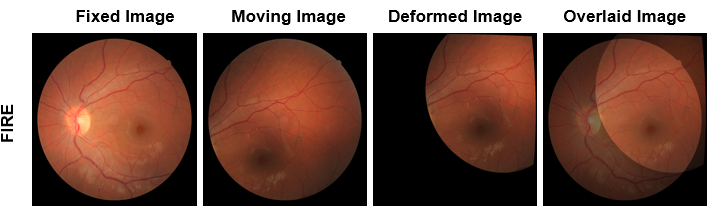
\includegraphics[width=0.8\textwidth]{imaxes/retin-reg.png}
    \caption{Ejemplo de registro de imágenes de retina \cite{sivaraman2024retinaregnetzeroshotapproachretinal}}
    \label{fig:retin_reg}
\end{figure}

\subsection{Categorías de registro}\label{subsec:Categorías de registro}

El registro de imágenes puede ser clasificado en distintas categorías según sus características.

\begin{itemize}
    \item \textbf{Según el número de imágenes:}
    \begin{itemize}
        \item \textit{Par a par:} El registro se realiza entre dos imágenes, una fija y una móvil.
        \item \textit{Múltiple:} Se registran varias imágenes simultáneamente, buscando una correspondencia global.
    \end{itemize}

    \item \textbf{Según la modalidad:}
    \begin{itemize}
        \item \textit{Intra-modalidad:} Las imágenes pertenecen a la misma modalidad (por ejemplo, dos retinografías).
        \item \textit{Inter-modalidad:} Las imágenes provienen de modalidades diferentes (por ejemplo, retinografía y OCT).
    \end{itemize}

    \item \textbf{Según el tipo de transformación:}
    \begin{itemize}
        \item \textit{Rígida:} Solo permite traslación y rotación, manteniendo las distancias y ángulos.
        \item \textit{Afín:} Además de traslación y rotación, permite escalado y cizallamiento.
        \item \textit{Deformable (no rígida):} Permite deformaciones locales complejas y no lineales.
        \item \textit{Difeomórfica:} Transformación no rígida que es continua, invertible y diferenciable en todo su dominio. Si no tiene esta característica, no se puede garantizar que la transformación sea reversible, por lo que son preferidas en muchos casos \cite{han2022diffeomorphicimageregistrationneural}.
    \end{itemize}

    \item \textbf{Según el grado de automatización:} \cite{deeplernreview3dreg}
    \begin{itemize}
        \item \textit{Manual:} El usuario selecciona puntos de control o ajusta parámetros.
        \item \textit{Automático:} El proceso se realiza sin intervención humana, mediante algoritmos.
        \item \textit{Semiautomático:} Combina intervención manual y automática.
    \end{itemize}

    \item \textbf{Según la naturaleza de la transformación:}
    \begin{itemize}
        \item \textit{Simétrico:} La transformación es consistente en ambas direcciones entre las imágenes.
        \item \textit{Asimétrico:} La transformación se calcula solo en un sentido. Cuando se trabaja con imágenes de forma asimétrica, la imagen de referencia se denomina imagen fija y la imagen que se quiere registrar imagen móvil.
    \end{itemize}

\end{itemize}

Las transformaciones lineales globales suelen representarse en matrices de transformación, donde cada elemento de la matriz representa un parámetro de la transformación.

En el caso de transformaciones más complejas, se utilizan campos de vectores de deformación (\gls{DFV}s), que permite representar deformaciones locales en la imagen, haciéndola mucho más flexible para representar transformaciones no lineales y detalladas.
Los DFVs suelen ser representados con una matriz de igual tamaño a la imagen, donde cada elemento representa un vector que indica la dirección y la magnitud de la deformación.

Este trabajo se ubica en el registro de imágenes par a par, intra-modalidad y con transformaciones deformables. Es un proceso totalmente automático que produce transformaciones asimétricas.

En la figura \ref{fig:dfv_visualization} se muestran dos formas de visualizar un DFV: mediante flechas que indican la dirección y magnitud de la deformación, y aplicando la deformación a una cuadrícula para ver cómo se distorsiona.

\begin{figure}[tbp]
    \centering
    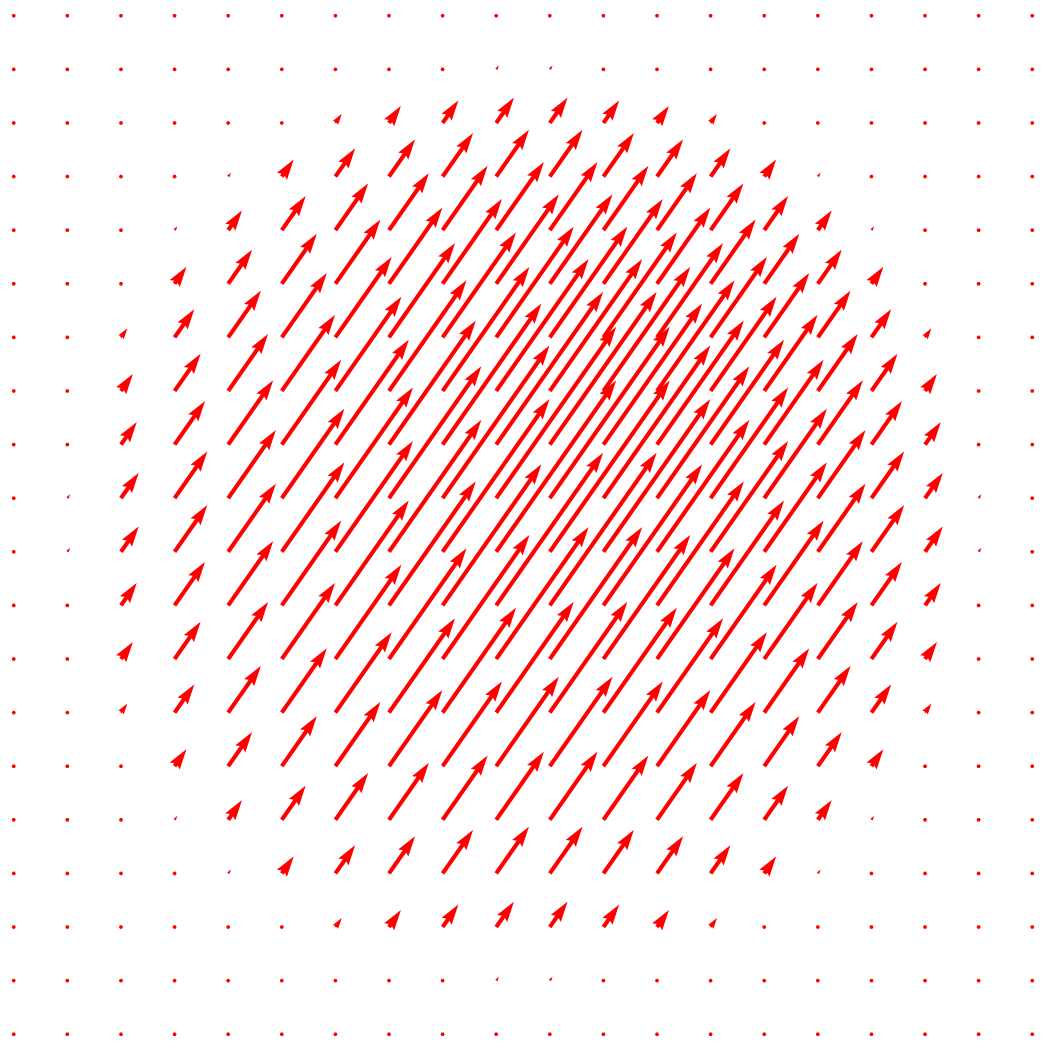
\includegraphics[width=0.45\textwidth]{imaxes/dfv_arrows.png}
    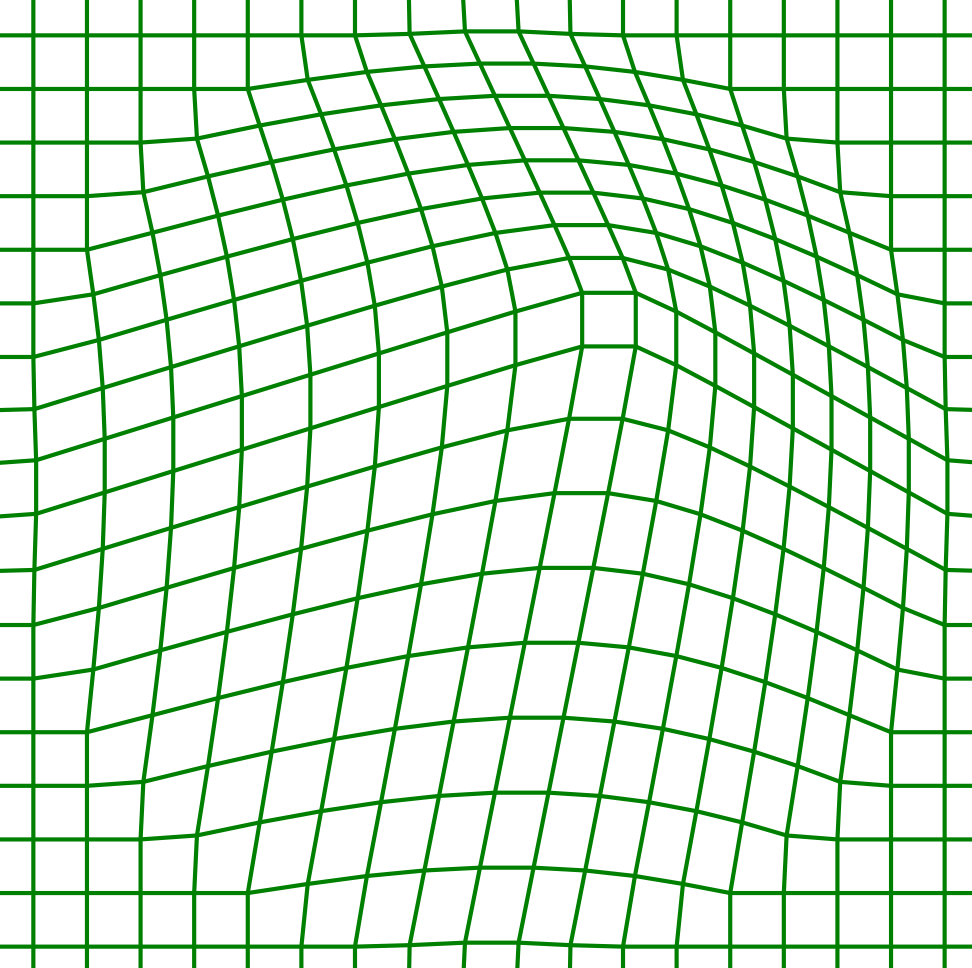
\includegraphics[width=0.45\textwidth]{imaxes/dfv_grid.png}
    \caption{Visualización del campo de vectores de deformación (DFV). A la izquierda, representación mediante flechas. A la derecha, esta deformación aplicada a una cuadrícula.}
    \label{fig:dfv_visualization}
\end{figure}

\subsection{Estado del arte}
\label{subsec:Estado del arte}

El registro de imágenes médicas constituye un área de investigación fundamental que ha experimentado importantes avances en las últimas décadas. En este ámbito, la precisión y la robustez del registro cobran especial relevancia, ya que son empleados para el diagnóstico y seguimiento de enfermedades, así como para la planificación de tratamientos quirúrgicos.
En el campo de la oftalmología, los métodos que funcionan bien en varios dominios de imagen médica (cerebro, pulmones, etc) suelen requerir ajustes para funcionar en retinas, por lo que hay un estado del arte paralelo.

La evolución de los métodos de registro en retinografías refleja la transición desde enfoques puramente algorítmicos hacia metodologías híbridas, donde publicaciones recientes como HybridRetina \cite{liu2024progressiveretinalimageregistration} muestran cómo para alcanzar los mejores resultados es beneficioso combinar ambos enfoques, aprovechando la precisión de los métodos clásicos y la adaptabilidad de los métodos de aprendizaje automático.

\subsubsection{Métodos clásicos}\label{subsubsec:Métodos clásicos}

Los métodos clásicos de registro de imágenes médicas pueden clasificarse en dos categorías principales:
Aquellos basados en similitud de imagen (\gls{IBR}) y aquellos basados en características (\gls{FBR}).
También existen métodos híbridos que combinan ambos enfoques \cite{integrateintfeat}.
El resultado final puede ser los parámetros de la transformación o la imagen fusionada.

\paragraph{Métodos basados en similitud de imagen}
\label{par:Métodos basados en similitud de imagen}

El registro se realiza comparando los valores de intensidad de los píxeles o voxeles mediante una métrica de similitud entre la imagen fija y la imagen móvil.
Este enfoque tiende a requerir múltiples iteraciones para converger, en las cuales se calcula el grado de semejanza entre las imágenes y
se actualizan los parámetros de la transformación utilizando un mecanismo de optimización hasta que se cumplan los criterios de terminación.

Los métodos de registro tradicionales tienen tres componentes principales: la métrica de similitud, el optimizador y el modelo de transformación.

La figura \ref{fig:rexistro_iterativo} muestra un diagrama del proceso de registro iterativo.

\paragraph{Métodos basados en características}
\label{par:Métodos basados en características}

El registro se realiza identificando y emparejando características destacables entre las imágenes, como puntos, líneas o bordes.
Típicamente, estos métodos tienen 3 pasos principales:

\begin{itemize}
\item \textbf{Detección de puntos de interés:} Identificación de puntos o regiones destacables en las imágenes, como bordes, esquinas o texturas. Para esto pueden utilizarse algoritmos como SIFT \cite{sift}, SURF \cite{surf}, BRISK \cite{brisk} o FREAK \cite{freakkeypoint}.
\item \textbf{Descripción de características:} los puntos detectados son descritos y comparados entre imágenes usando descriptores.
\item \textbf{Estimación de la transformación:} una vez encontradas las correspondencias, se calcula la transformación que alinea las imágenes con algoritmos de emparejamiento como FLANN \cite{flann} o RANSAC \cite{ransac}.
\end{itemize}

Algunos de los métodos tradicionalmente más utilizados en este campo son \gls{GDB-ICP} \cite{GDB-ICP} y Harris-PIIFD \cite{piifd}. Este último utiliza el algoritmo Harris \cite{Harris1988ACC} para la detección de puntos de interés, los describe con \gls{PIIFD}, y se emparejan usando \gls{BBF} \cite{BBF}.
Finalmente, se refinan las coincidencias y se elige la transformación (rígida, afín o polinomial) según el número de pares de puntos válidos. Sobre esta base se han propuesto varias mejoras para adaptarlo al registro multimodal de retinas como UR-SIFT \cite{ur-sift} o \gls{GMM} \cite{GMM}.

Una ventaja de este enfoque es la capacidad para registrar imágenes con grandes variaciones locales o modalidades diferentes, ya que no depende tanto de la semejanza global entre las imágenes.

Otros métodos clásicos relevantes en el campo de la imagen de ojo incluyen REMPE \cite{rempe}, que estima simultáneamente la pose de las cámaras y la forma del ojo. Hace uso de un modelo elipsoidal para el ojo y estima la posición de las cámaras con RANSAC, para luego refinarla con una variante de PSO \cite{pso}.

\begin{figure}[tbp]
\centering
\begin{tikzpicture}[node distance=2cm, scale=0.8, every node/.style={transform shape}]
% Nodes
\node (imageFixa) [process] {Imagen Fija};
\node (imageMobil) [process, right of=imageFixa, xshift=3cm] {Imagen Móvil};
\node (featureExtraction) [process, below of=imageFixa, yshift=-1cm] {Cálculo de medida de similitud};
\node (parameterUpdate) [process, below of=featureExtraction, yshift=-1cm] {Actualización de Parámetros};
\node (applyTransformation) [process, below of=parameterUpdate, yshift=-1cm] {Aplicar la Transformación};
\node (criteriaCheck) [decision, below of=applyTransformation, yshift=-1cm] {¿Criterios Cumplidos?};
\node (result) [process, below of=criteriaCheck, yshift=-1cm] {Resultado};
% Arrows
\draw [arrow] (imageFixa) -- (featureExtraction);
\draw [arrow] (imageMobil) -- (featureExtraction);
\draw [arrow] (featureExtraction) -- (parameterUpdate);
\draw [arrow] (parameterUpdate) -- (applyTransformation);
\draw [arrow] (applyTransformation) -- (criteriaCheck);
\draw [arrow] (criteriaCheck) -- node[anchor=west] {Sí} (result);
\draw [arrow] (criteriaCheck.east) -- ++(1,0) node[anchor=south, xshift=0.5cm] {No} |- (featureExtraction.east);
\end{tikzpicture}
\caption{Proceso de registro de imágenes iterativo}
\label{fig:rexistro_iterativo}
\end{figure}

También existen múltiples programas que hacen uso de estos métodos en herramientas para facilitar el registro de imágenes, como SimpleITK \cite{simpleitk}, Elastix \cite{elastix} o ANTs \cite{ants}.

\subsubsection{Métodos de aprendizaje profundo}\label{subsubsec:Métodos de aprendizaje profunda}

Con la llegada de los métodos de aprendizaje profundo a la imagen médica, comenzaron a emplearse redes neuronales para realizar el alineamiento de imágenes.
Existe un gran interés por los métodos basados en aprendizaje profundo, como se refleja en el creciente número de publicaciones en el campo. En la figura \ref{fig:method_comp} se muestra la evolución del número de publicaciones sobre registro de imágenes, diferenciando entre los métodos basados en aprendizaje profundo y los métodos tradicionales.

Los métodos de aprendizaje profundo pueden ser clasificados en dos tipos según si requieren de \glossary{DFV}s anotados o no en la etapa de entrenamiento:
supervisados (requieren anotaciones) y no supervisados (no requieren anotaciones) \cite{nie2024medicalimageregistrationapplication}.

Según el grado de supervisión utilizado en la etapa de entrenamiento, los métodos supervisados pueden dividirse en supervisados o débilmente supervisados.
El registro totalmente supervisado hace uso de DVFs de referencia para supervisar el proceso de aprendizaje, y el término de pérdida suele basarse en la discrepancia entre los DVFs de referencia y los DVFs predichos.

El registro débilmente supervisado puede utilizar otras etiquetas de referencia implícitas, no basadas en datos explícitos como los DFVs, sino que utilizan información indirecta para guiar el proceso de registro, como la similitud entre las imágenes o restricciones basadas en la forma o límites anatómicos de las estructuras.
Más de dos tipos de datos de referencia son frecuentemente utilizados para entrenar modelos de registro débilmente supervisados \cite{bharati2022deeplearningmedicalimage}.

Los métodos no supervisados tienen la ventaja de no requerir datos anotados, lo cual es una gran ventaja ya que uno de los mayores retos para las redes de imágenes médicas es la recolección de datos de calidad para el entrenamiento \cite{medicalimageanalysis}.
La creación de conjuntos de DFVs anotados es un proceso laborioso y costoso, que normalmente solo puede ser ejecutado por especialistas, por lo que los métodos de registro no supervisados son de gran interés.
De forma similar a los métodos iterativos, es común emplear una métrica de similitud entre las imágenes junto con un término de regularización para guiar el proceso de optimización evitando caer en transformación no realistas.

Los enfoques de aprendizaje profundo son útiles tanto en su capacidad de aprender la tarea de registro de manera end-to-end, como para sustituir módulos concretos del proceso tradicional.
En ese sentido, los métodos de aprendizaje profundo pueden ser categorizados según la tarea del proceso de registro que sustituyen.

\begin{figure}[tbp]
\centering
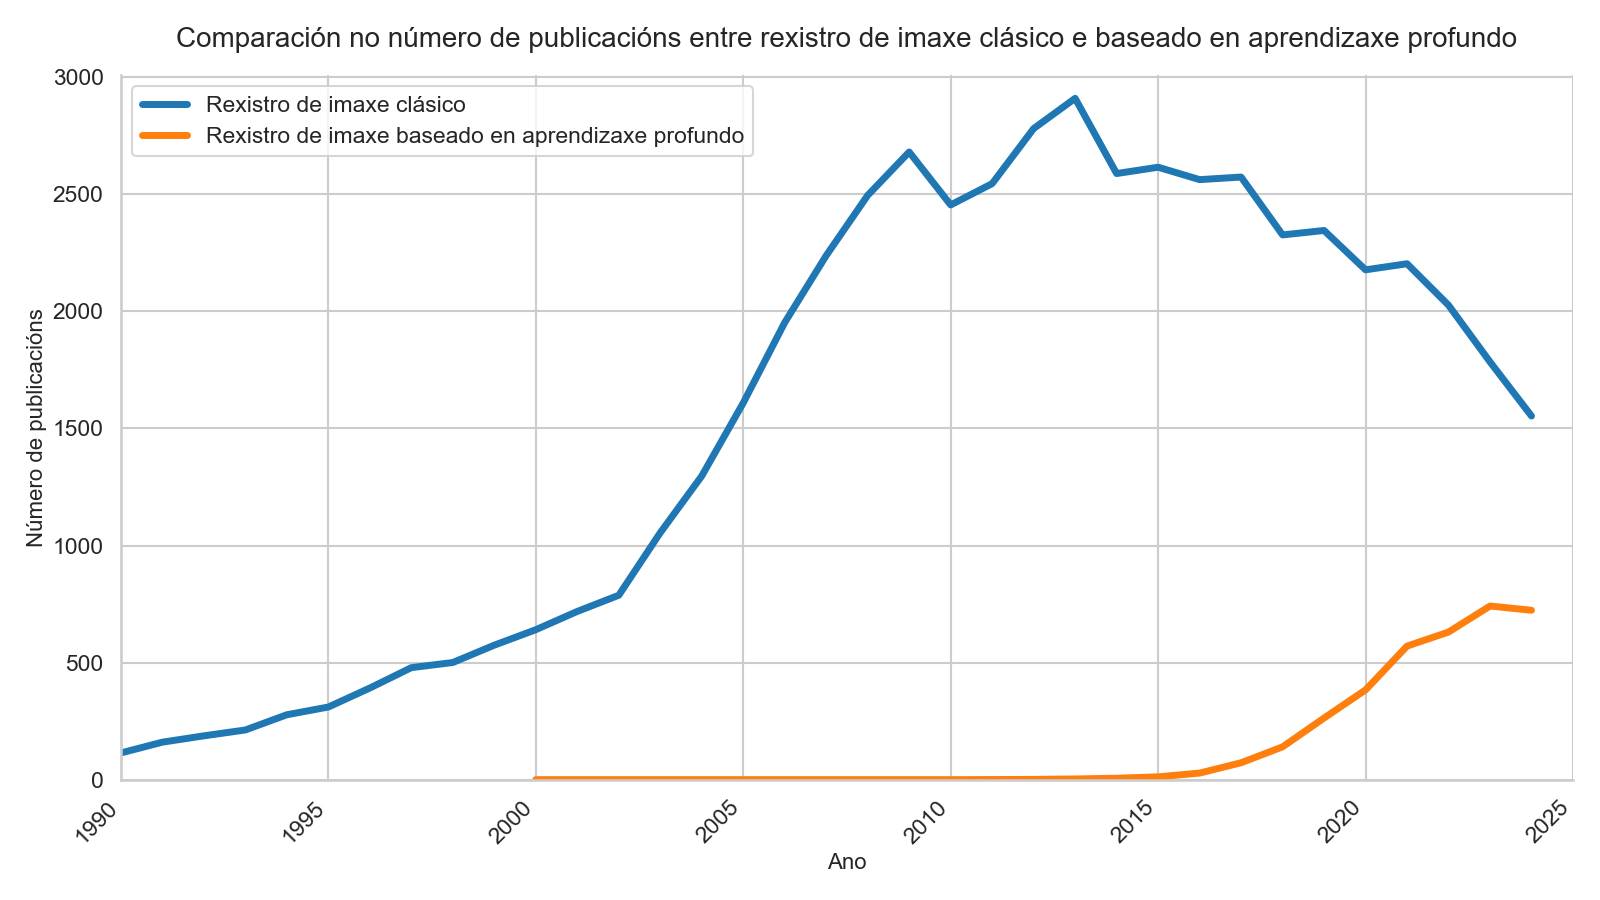
\includegraphics[width=0.8\textwidth]{imaxes/methods_comp.png}
\caption{Comparación de publicaciones a lo largo del tiempo relacionadas con el registro de imágenes. Datos extraídos de Scopus \cite{scopus}, realizando las consultas: "TITLE-ABS-KEY(image AND registration) AND NOT(deep AND learning)" y "TITLE-ABS-KEY(image AND registration) AND (deep AND learning)"}
\label{fig:method_comp}
\end{figure}

Los métodos de aprendizaje profundo pueden sustituir cualquiera de estos pasos que forman los métodos de registro clásicos de forma independiente o en combinación.

\paragraph{En registro basado en intensidad (IBR)}
\label{par:IBR_substitution}

\begin{itemize}
\item \textbf{Métrica de similitud:} Los métodos de aprendizaje profundo pueden aprender métricas de similitud más robustas que las tradicionales. Estas métricas aprendidas pueden ser más efectivas en imágenes multimodales o con artefactos.
Por ejemplo, Czolbe et al. \cite{semanticsimilarity} proponen dos métricas de similitud semánticas que aprende la semejanza entre imágenes comparando las características de alto nivel extraídas. Presentan una aproximación no supervisada que hace uso de autoencoders y otra semisupervisada que incorpora datos de segmentación.
\item \textbf{Optimizador:} Los métodos de aprendizaje profundo pueden sustituir el proceso de optimización iterativa tradicional por redes que aprenden a predecir directamente los parámetros de transformación óptimos. Una aproximación común es emplear estos conjuntos de datos para optimizar una CNN que, dadas dos imágenes nuevas y no vistas, predice el DFV correspondiente \cite{defregcnn}. Durante el proceso de entrenamiento, la red puede tener acceso a los DFVs con la deformación correcta, o se pueden obtener indirectamente a través de la optimización de una métrica de similitud de imágenes.
\item \textbf{Modelo de transformación:} Estos métodos aprenden representaciones implícitas de la transformación a través de redes neuronales, permitiendo modelar deformaciones más complejas que los modelos paramétricos tradicionales. Los métodos como IDIR \cite{wolterink2021implicit} encajan en esta categoría, utilizando campos neuronales implícitos para representar las transformaciones de registro.
\end{itemize}

\paragraph{En registro basado en características (FBR)}
\label{par:FBR_substitution}

\begin{itemize}
\item \textbf{Detectores de características:} Las redes neuronales pueden aprender a detectar puntos de interés más robustos y repetibles que los detectores clásicos como \glossary{SIFT}. SuperPoint \cite{superpoint} introduce un detector de características basado en redes neuronales que aprende a detectar puntos de interés y a describirlos simultáneamente.
\item \textbf{Descriptores de características:} Los descriptores aprendidos mediante redes neuronales pueden capturar información más discriminativa, mejorando la precisión del emparejamiento posterior. Estos métodos aprenden representaciones que son invariantes a transformaciones específicas del dominio.
\item \textbf{Emparejamiento:} Las redes neuronales pueden aprender a realizar el emparejamiento de características de forma robusta, especialmente en presencia de cambios de iluminación o perspectiva. SuperGlue \cite{superglue} es un ejemplo de modelo que aprende a emparejar puntos de interés detectados utilizando una arquitectura basada en atención para capturar las relaciones entre los puntos.
\end{itemize}

\paragraph{Métodos de regresión directa}
\label{par:direct_regression}

El aprendizaje profundo tiende a requerir de una gran cantidad de datos para ser entrenados, lo que puede ser una desventaja ya que en muchos casos no se disponen de bases de datos anotadas del tamaño necesario.

Los métodos de regresión directa aprenden a mapear directamente desde un par de imágenes hasta los parámetros de la transformación, sin necesidad de optimización iterativa ni extracción explícita de características.

También son denominados métodos de inferencia amortizada debido a la capacidad de realizar múltiples inferencias (registros) tras un único proceso de entrenamiento, en contraposición a los métodos tradicionales que requieren optimización individual para cada par de imágenes.
Estos enfoques son útiles por su eficiencia computacional en la fase de inferencia. Voxelmorph \cite{Balakrishnan_2019voxelmorph} es uno de los frameworks más utilizados en el registro de imágenes deformable, haciendo uso de modelos basados en \gls{CNN}s y que también permite incorporar información auxiliar (como segmentaciones) si está disponible, mejorando así la precisión del registro.

Métodos como UDIR-Net \cite{undefreg} o DIO \cite{Jena_2025} también implementan estas ideas.

\subsubsection{Estado del arte en el registro de retinografías}\label{subsubsec:Estado_da_arte_no_rexistro_de_retinografías}

El registro de retinografías presenta un conjunto de desafíos únicos que lo distinguen de otros dominios de la imagen médica.
Uno de los principales obstáculos son las deformaciones no rígidas. Estas deformaciones pueden originarse por la proyección de la superficie 3D curva de la retina en una imagen 2D o variaciones en la forma del ojo de cada paciente. Además, es frecuente encontrar pares de imágenes con áreas de solapamiento mínimas lo que dificulta la identificación de correspondencias para el alineamiento. A esto se suman las variaciones de iluminación, contraste y color entre imágenes capturadas en diferentes situaciones, así como los cambios anatómicos inducidos por patologías, que alteran las estructuras utilizadas para el registro.
Finalmente, la escasez de conjuntos de datos públicos, especialmente para condiciones o poblaciones específicas, supone una barrera importante para el desarrollo de modelos de aprendizaje supervisado.

La dificultad para obtener campos de deformación de referencia para el entrenamiento impulsó el desarrollo de marcos no supervisados. Estos modelos se entrenan optimizando una función de pérdida basada en la similitud de imagen entre la imagen móvil deformada y la imagen fija, junto con un término de regularización sobre la suavidad de la deformación.

Dentro de los métodos clásicos, los basados en características (FBR) siguen siendo referentes en cuanto a precisión. Entre ellos destacan VOTUS \cite{Votus}, que es especialmente robusto en imágenes de poco solapamiento y representa los árboles vasculares como grafos para encontrar la correspondencia entre ellos. REMPE \cite{rempe} es otro método ya mencionado anteriormente en esta categoría.

En el campo del aprendizaje profundo, RetinaRegNet \cite{sivaraman2024retinaregnetzeroshotapproachretinal} es un modelo reciente de tipo "zero-shot" que utiliza características extraídas de modelos de difusión para establecer correspondencias, alcanzando resultados de vanguardia.

ConKeD (Contrastive Keypoint Descriptors) y su evolución, ConKeD++, se centran en perfeccionar la creación de descriptores de puntos de interés, uno de los componentes más críticos de los métodos basados en características (FBR).
La principal ventaja es que obtiene resultados comparables a los de los métodos clásicos de vanguardia (como REMPE y VOTUS) pero con tiempos de ejecución mucho más rápidos.

La mayoría de estos algoritmos son evaluados y comparados utilizando el conjunto de datos de referencia FIRE \cite{FIRE}, permitiendo una cuantificación objetiva del rendimiento.

\section{Representaciones Neuronales Implícitas}
\label{sec:Representación Neuronais Implícitas}

La representación de conocimiento es uno de los problemas más importantes en el área de la computación, y las redes profundas son una de las herramientas más útiles, especialmente en el campo de la visión por computador.
Tradicionalmente se emplean representaciones discretas, donde el espacio de entrada es dividido en celdas y cada celda es asignada un valor (por ejemplo nubes de puntos, matrices de píxeles o vóxeles...).
Una de las principales desventajas de estas representaciones es que su complejidad se incrementa rápidamente con el número de dimensiones representadas, además del coste de memoria asociado.

Las representaciones neuronales implícitas son un paradigma innovador que permite modelar señales continuas mediante funciones parametrizadas por redes neuronales.
Codifican la información como una función continua, que mapea valores de entrada a los valores correspondientes de salida, en lugar de almacenar directamente valores de características o señales.

Representar la señal como una función continua permite solucionar los problemas asociados a la discretización y se obtienen otra serie de ventajas.

Las INR son mucho más eficientes debido a la compresión de la información que realizan de forma implícita. Al mismo tiempo, permite un nivel de detalle no limitado por la resolución de la imagen, sino por la capacidad de la red.
Además, las representaciones continuas son diferenciables, lo que permite el cálculo de gradientes y derivadas de forma analítica en lugar de tener que aproximarlos por diferencias finitas.
Esto también implica que las representaciones implícitas son independientes de la resolución, lo que permite la reconstrucción en cualquier escala espacial.

Típicamente se emplea un MLP como arquitectura para representar la función implícita. No obstante, el uso de la función de activación ReLU tiende a no obtener los mejores resultados, debido a que son incapaces de representar deformaciones locales sin afectar a su comportamiento global \cite{rahaman2019spectralbiasneuralnetworks},
por lo que mucha investigación se dirige a encontrar alternativas que mejoren la representación de la señal. \cite{essakine2024standimplicitneuralrepresentations}

Una de estas alternativas es SIREN \cite{sitzmann2020implicitneuralrepresentationsperiodic}, sobre la que profundizaremos más adelante.
Otras propuestas incluyen \cite{ramasinghe2022periodicityunifyingframeworkactivations} propone las funciones de activación gaussianas como alternativa a SIREN, y argumenta que pueden obtener mejores representaciones y más robustas.
\cite{saragadam2023wirewaveletimplicitneural} aporta una nueva función de activación basada en wavelets, que parece ser especialmente útil para la representación de imágenes.

Las representaciones implícitas pueden ser clasificadas en dos categorías: generalizables y sobreajustadas \cite{yu2024neuraltrajectorymodelimplicit}.
Las representaciones sobreajustadas se centran en reproducir con precisión una única señal, mientras que las representaciones generalizables pueden modelar varias en una misma red.

\subsection{Aplicaciones}
\label{subsec:Aplicacións}

Las INR son utilizadas en todo tipo de campos, desde generación de imágenes \cite{reddy2022multiimplicitneuralrepresentationfonts}, pasando por
reconstrucción de objetos \cite{mildenhall2020nerfrepresentingscenesneural} \cite{mescheder2019occupancynetworkslearning3d} o modelado de señales complejas \cite{wu2021iremhighresolutionmagneticresonance}.

Las representaciones implícitas están recibiendo cada vez más atención de la comunidad médica, y son especialmente útiles para las tareas de imagen inversa, que requieren la reconstrucción de representaciones correctas a partir de datos incompletos o ruidosos \cite{molaei2023implicitneuralrepresentationmedical}.
Métodos como NeRP, propusieron el uso de representaciones implícitas para la reconstrucción de imágenes de resonancia magnética a partir de datos incompletos, y obtuvieron resultados comparables a métodos tradicionales \cite{shen2023nerpimplicitneuralrepresentation}.

NeRF hace uso de representaciones implícitas para sintetizar nuevos puntos de vista en escenas 3D \cite{mildenhall2020nerfrepresentingscenesneural},
optimizando una función volumétrica continua que modela la densidad de volumen y la radiancia emitida en cada punto del espacio.
Utilizan un MLP, cuya entrada es una única coordenada continua 5D (localización espacial (x, y, z) y dirección de visión (θ, φ))
y cuya salida es la densidad de volumen y la radiancia emitida dependiente de la vista en esa localización espacial.
La única entrada necesaria para optimizar su representación es un conjunto de imágenes con poses de cámara conocidas.
Este trabajo demuestra que las representaciones implícitas están capacitadas para modelar escenas 3D complejas con alta fidelidad visual.

Las representaciones implícitas también tienen bastante potencial en el campo de planificación de trayectorias,
donde se hace uso de INRs para modelar entornos y planificar trayectorias para uno o varios agentes \cite{yu2024neuraltrajectorymodelimplicit}.
La principal ventaja de hacerlo de esta forma frente a la forma tradicional (algoritmos computacionalmente intensos, especialmente para multi-agentes) es la velocidad a la que encuentran soluciones (por debajo del milisegundo en GPUs).
La mayor desventaja es que no garantizan la convergencia a una solución óptima y sin colisiones, pero los autores demuestran que la calidad de las trayectorias generadas es adecuada para la mayoría de las aplicaciones \cite{trajectinr}.

En el ámbito médico, se utilizan este tipo de representaciones para garantizar la seguridad del paciente durante la cirugía teleoperada y optimizar la trayectoria del robot para evitar colisiones con el paciente, por ejemplo en la boca y garganta \cite{teleoperatdrob}.
Con este método, se evita la reconstrucción de mallas a partir de imágenes, que es un proceso costoso e imperfecto, y se modela mediante una INR a partir de los datos médicos disponibles.
Los comandos de movimiento de la mano del operador son tomados como entrada por el modelo, que después de un proceso de optimización, genera una secuencia de movimientos libre de colisiones que será enviada a la mano robótica.
También son utilizadas para crear reconstrucciones 3D de pulmones que mitigan las distorsiones causadas por el movimiento respiratorio \cite{velikova2024implicitneuralrepresentationsbreathingcompensated}.

Otro uso interesante de las representaciones neuronales implícitas es la compresión de imágenes. Algoritmos como COIN \cite{coin} representan los datos de entrada mediante redes neuronales implícitas (funciones que mapean coordenadas a valores RGB), logrando una compresión eficiente y una reducción significativa del tiempo de codificación en muchas modalidades.

\subsection{Registro basado en Representaciones Neuronales Implícitas}\label{subsec:Rexistro_baseado_en_INRs}

El registro de imágenes basado en Representaciones Neuronales Implícitas (INR) parametriza la transformación de deformación como una función continua, generalmente con un Perceptrón Multicapa (MLP), que mapea coordenadas espaciales a vectores de desplazamiento. A diferencia de las CNN, la red no procesa las intensidades de la imagen directamente, sino que se optimiza usando estas para calcular la pérdida. Una de las ventajas en este contexto es la capacidad de calcular gradientes analíticos exactos de la transformación, permitiendo una regularización más precisa que con aproximaciones de los métodos basados en rejillas.

Las funciones de activación periódicas (SIREN \cite{sitzmann2020implicitneuralrepresentationsperiodic}) permitieron superar el problema de los sesgos hacia transformaciones de baja frecuencia del MLP, y fueron utilizadas por IDIR alcanzando resultados de vanguardia \cite{wolterink2021implicit}.

Los principales inconvenientes son la lentitud en la inferencia (requiere optimización para cada par de imágenes) y la tendencia a generar pliegues espaciales (deformaciones no realistas). La investigación actual se centra en modelos híbridos para mitigar estos problemas.
Algunos de los enfoques más relevantes incluyen:
SINR (Spline-enhanced INR) combina INR con B-splines, donde la red predice los desplazamientos de una rejilla de control dispersa. Esto impone suavidad de forma intrínseca y facilita el registro multimodal \cite{SINR}.
INR ciclo-consistentes, que entrenan simultáneamente la transformación directa y la inversa, usando cada red como regularizador de la otra para mejorar la robustez.
Meta-aprendizaje: Aprende una inicialización de pesos óptima a partir de un gran conjunto de datos para acelerar drásticamente la convergencia en la inferencia \cite{learnedinit}.
INR condicionadas por geometría: Incorporan conocimiento anatómico previo para simplificar la complejidad de la deformación a aprender \cite{harten2023deformable}.
Sun et al. \cite{sun2024medicalimageregistrationneural} proponen un registro de imágenes que usa campos neuronales para modelar la transformación, utilizando también codificación posicional (que transforma las coordenadas espaciales en vectores de alta dimensión) lo que permite que la red aprenda con mayor facilidad las transformaciones de alta frecuencia.

El uso de Representaciones Neuronales Implícitas (INR) para el registro de imágenes ofrece una precisión notable al modelar la deformación como una función continua y analíticamente diferenciable. Este enfoque, ejemplificado por el éxito inicial de IDIR, permite una regularización más exacta que los métodos basados en rejillas. No obstante, su aplicación práctica se ve obstaculizada por la lentitud de la optimización por cada par de imágenes y el riesgo de producir deformaciones no realistas con pliegues espaciales. El estado del arte actual tiende a abordar estos retos mediante la hibridación.

\section{Trabajo propuesto}
\label{sec:Traballo proposto}

El trabajo propuesto se ubica dentro de los métodos de aprendizaje profundo, y más concretamente en el registro de imágenes basado en intensidad (IBR) utilizando representaciones neuronales implícitas (INRs).

Como mostramos en este capítulo, a pesar del potencial de las representaciones neuronales implícitas en diversos dominios médicos, su aplicación específica al registro de retinografías permanece inexplorada.

Esta falta de investigación es especialmente relevante dadas las potenciales ventajas que ofrecen las INRs, como la capacidad de modelar deformaciones complejas y su independencia de la resolución.

Basándose en el framework introducido por \cite{wolterink2021implicit}, se propone modificarlo para adaptarlo a la tarea de registro de retinografías. El objetivo es conseguir registros consistentemente precisos, especialmente en el dataset de FIRE que contiene imágenes reales de retina.

Esta adaptación representa una contribución novel al estado del arte en el registro de retinografías, explorando por primera vez el potencial de las representaciones neuronales implícitas en este dominio específico.